\documentclass[../../../../main.tex]{subfiles}

\begin{document}

\section*{東大理科数学 2001年}

\begin{center}
\begin{tabular}{|c|c|c|c|c|}
\hline
問 & 分野 & 思 & 計 & 総 \\ \hline
1 & 空間 & B & B & B \\ \hline
2 & 多変数 & C & B & B \\ \hline
3 & 多変数(関数?) & A & B & B \\ \hline
4 & 複素数 & B & B & B \\ \hline
5 & 論理 & C & A & C \\ \hline
6 & 場合の数 & B & B & B \\ \hline
\end{tabular}
\end{center}

\bigskip

\subsection*{第1問}

\begin{center}
\begin{tabular}{|l|}
\hline
\textbf{[球・円]} \\
・中心を含む平面で切る (対称性) \\
\hline
\end{tabular}
\end{center}

\noindent
—— \textbf{[等式のとき方 - パート②]} —— \\
まとまったカタマリを文字でおく手法

\bigskip

\noindent
\textbf{[解]}
題意の球の中心を $O$ とする。$CD$ の中点を $E$ とし $\triangle ABE$ で切断すると、右図。対称性から、$O$ は $\triangle ACD$ の外心を通り $\triangle ACD$ に垂直な直線上かつ $\triangle BCD$ の外心を通り $\triangle BCD$ に垂直な直線上にあることをあわせて、この平面上にある。$O$ から $AE, BE$ に下ろした垂足を $P, Q$ とすると、

\begin{center}
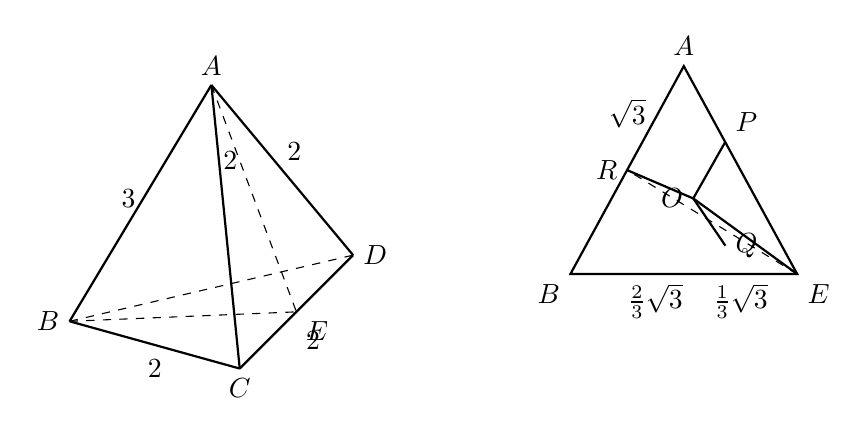
\begin{tikzpicture}[scale=1.2, >=stealth]
  % Tetrahedron diagram (left)
  \coordinate (A) at (0, 2);
  \coordinate (B) at (-1.5, -0.5);
  \coordinate (C) at (0.3, -1);
  \coordinate (D) at (1.5, 0.2);
  \coordinate (E) at (0.9, -0.4);

  \draw[thick] (A) -- (B) node[left] {$B$};
  \draw[thick] (A) -- (C);
  \draw[thick] (A) -- (D) node[right] {$D$};
  \draw[thick] (B) -- (C) node[below] {$C$};
  \draw[thick] (C) -- (D);
  \draw[dashed] (B) -- (D);
  \draw[dashed] (A) -- (E) node[below right] {$E$};
  \draw[dashed] (B) -- (E);

  \node[above] at (A) {$A$};
  \node[left] at (-0.7, 0.8) {$3$};
  \node[above right] at (0.7, 1.1) {$2$};
  \node[below] at (-0.6, -0.8) {$2$};
  \node[right] at (0.9, -0.7) {$2$};
  \node[above] at (0.2, 1) {$2$};

  % Cross-section diagram (right)
  \begin{scope}[xshift=5cm]
    \coordinate (A2) at (0, 2.2);
    \coordinate (B2) at (-1.2, 0);
    \coordinate (E2) at (1.2, 0);
    \coordinate (R) at (-0.6, 1.1);
    \coordinate (O) at (0.1, 0.8);
    \coordinate (P) at (0.44, 1.4);
    \coordinate (Q) at (0.44, 0.3);

    \draw[thick] (A2) node[above] {$A$} -- (B2) node[below left] {$B$} -- (E2) node[below right] {$E$} -- cycle;
    \draw[dashed] (E2) -- (R) node[left] {$R$};
    \draw[thick] (O) node[left] {$O$} -- (P) node[above right] {$P$};
    \draw[thick] (O) -- (Q) node[right] {$Q$};
    \draw[thick] (O) -- (R);
    \draw[thick] (O) -- (E2);

    \node[left] at (-0.3, 1.7) {$\sqrt{3}$};
    \node[below] at (-0.3, 0) {$\frac{2}{3}\sqrt{3}$};
    \node[below] at (0.6, 0) {$\frac{1}{3}\sqrt{3}$};
  \end{scope}
\end{tikzpicture}
\end{center}

\noindent
したがって、
\[
\bar{AP} = \bar{BQ} = \frac{2}{3}\sqrt{3} \quad \cdots \textcircled{1}
\]
となる。$O$ から $AB$ に下ろした垂足を $R$ とする。
\[
\bar{ER} = \frac{3}{2} \quad \cdots \textcircled{2}
\]
\[
\bar{OR} = \sqrt{r^2 - \left(\frac{3}{2}\right)^2} = \sqrt{r^2 - \frac{9}{4}} \quad \cdots \textcircled{3} \quad (\because \textcircled{2})
\]
\[
\bar{OE} = \sqrt{\bar{OP}^2 + \left(\frac{1}{3}\sqrt{3}\right)^2} = \sqrt{\left\{r^2 - \left(\frac{2}{3}\sqrt{3}\right)^2\right\} + \left(\frac{1}{3}\sqrt{3}\right)^2} = \sqrt{r^2 - 1} \quad \cdots \textcircled{4} \quad (\because \textcircled{1})
\]
\textcircled{2}～\textcircled{4}から、$\bar{ER}$ を2通りで表して ($E-O-R$ は一直線上)、
\[
\frac{3}{2} = \sqrt{r^2 - \frac{9}{4}} + \sqrt{r^2 - 1}
\]
$t = r^2$ として、両辺正から2乗して
\[
\frac{9}{4} = 2t - \frac{13}{4} + 2\sqrt{\left(t - \frac{9}{4}\right)(t - 1)}
\]
\[
2 - t = \sqrt{\left(t - \frac{9}{4}\right)(t - 1)}
\]
$t < 2$ のもとで2乗して
\[
-4t + 4 = -\frac{13}{4}t + \frac{9}{4}
\]
\[
t = \frac{13}{9} \quad (t < 2 \text{ をみたす})
\]
$r > 0$ から
\[
r = \sqrt{t} = \frac{\sqrt{13}}{3} \hfill \text{\slash\slash}
\]

\bigskip

\subsection*{第2問}

\noindent
\textbf{[解]} $S = \sin x, C = \cos x, S' = \sin y, C' = \cos y$ とする。又 $f(y) = f$ と略記する。
\[
\int_0^{2\pi} \sin(x+y) f(y) \, dy = S \int_0^{2\pi} C' f \, dy + C \int_0^{2\pi} S' f \, dy
\]
\[
\int_0^{2\pi} \cos(x-y) f(y) \, dy = C \int_0^{2\pi} C' f \, dy + S \int_0^{2\pi} S' f \, dy
\]
だから、与式に代入して、
\[
f = \left[ \frac{a}{2\pi} \int_0^{2\pi} C' f \, dy + \frac{b}{2\pi} \int_0^{2\pi} S' f \, dy + 1 \right] S + \left[ \frac{a}{2\pi} \int_0^{2\pi} S' f \, dy + \frac{b}{2\pi} \int_0^{2\pi} C' f \, dy + 1 \right] C \quad \cdots *
\]
だから、左の括弧内を $A$、右の括弧内を $B$ として
\[
f = A S + B C \quad \cdots \textcircled{3}
\]
と書ける。したがって、
\[
\int_0^{2\pi} S' f \, dx = \int_0^{2\pi} (A S^2 + B C S) \, dx = \frac{1}{2} A \left[ x - \frac{1}{2}\sin 2x \right]_0^{2\pi} - \frac{1}{4} B \left[ \cos 2x \right]_0^{2\pi} = A \pi \quad \cdots \textcircled{4}
\]
\[
\int_0^{2\pi} C' f \, dx = \int_0^{2\pi} (A S C + B C^2) \, dx = -\frac{1}{4} A \left[ \cos 2x \right]_0^{2\pi} + \frac{1}{2} B \left[ x + \frac{1}{2}\sin 2x \right]_0^{2\pi} = B \pi \quad \cdots \textcircled{5}
\]
とあわせて $A, B$ の定義式に代入すると、
\[
\begin{cases}
A = \frac{a}{2\pi} B \pi + \frac{b}{2\pi} A \pi + 1 = \frac{1}{2} a B + \frac{1}{2} b A + 1 \\
B = \frac{a}{2\pi} A \pi + \frac{b}{2\pi} B \pi + 1 = \frac{1}{2} a A + \frac{1}{2} b B + 1
\end{cases}
\]
\[
\therefore
\begin{cases}
(b-2)A + aB + 2 = 0 \\
aA + (b-2)B + 2 = 0
\end{cases}
\quad \cdots \textcircled{6}
\]
$(A,B) = (0,0)$ の時、\textcircled{6}は成立せず不適だから、$A, B$ のうち少なくとも一方は $0$ でない。したがって\textcircled{3}から、$(A,B)$ が一意に定まることが、$f$ が一意に定まることの必要十分条件である。$\cdots \textcircled{7}$

ここで、$AB$ 平面上で連立方程式\textcircled{6}の解は2直線の共有点を表すから、($(a,b) = (0,2)$ の時は不適だから、$a, b-2$ のうち少なくとも一方は $0$ でない)
\textcircled{6}の解が一意に定まるには、\textcircled{6}の2直線が平行でなければ良く、
\[
(b-2)^2 \neq a^2 \quad \cdots \textcircled{8}
\]
が条件である。(これは $(a,b) \neq (0,2)$ を含む) 以上\textcircled{7}、\textcircled{8}から、求める条件は
\[
(b-2)^2 \neq a^2 \hfill \text{\slash\slash}
\]
である。この時\textcircled{6}を解いて、$A = B = \frac{2}{2-(a+b)}$ だから、\textcircled{3}に代入して
\[
f(x) = \frac{2}{2-(a+b)} (\sin x + \cos x) \hfill \text{\slash\slash}
\]
である。

\bigskip

\noindent
\textbf{[後半部の別解]} \\
$k = b-2$ として、\textcircled{6}の2本の和差をとって
\[
\begin{cases}
(k+a)(A+B) = -4 & \cdots \textcircled{1}' \\
(k-a)(A-B) = 0 & \cdots \textcircled{2}'
\end{cases}
\]
\textcircled{6} $\iff$ \textcircled{1}' \textcircled{2}' に注意する。

\medskip

\noindent
$1^\circ \; k-a \neq 0$ \\
\textcircled{2}' から $A=B$ である。$k+a=0$ は不適だから、\textcircled{1}'より
\[
A = B = \frac{2}{2-(a+b)}
\]
この時、$f$ は一意に定まる。

\medskip

\noindent
$2^\circ \; k-a = 0$ \\
\textcircled{2}' は任意の $(A,B)$ で成立する。$k+a=0$ は不適だから、\textcircled{1}'から
\[
B = -A - \frac{2}{k+a}
\]
となり、$f$ は一意に定まらない。

\medskip

\noindent
以上から、求める条件は $b-2 \neq \pm a$ つまり $f(x) = \frac{2}{2-(a+b)}(\sin x + \cos x)$ である。

\bigskip

\subsection*{第3問}

\noindent
\textbf{[解]}
\[
a(t) = \frac{1}{2} \left| t - \frac{1}{t} \right| = \frac{1}{2} \left( t - \frac{1}{t} \right) \quad (\because t > 1) \quad \cdots \textcircled{1}
\]
とする。$P, Q$ から $x$ 軸に下ろした垂足を $P', Q'$ として
\[
b(t) = \triangle OPP' - \triangle OQQ' + \text{台形 } PP'Q'Q
\]
\[
= \frac{1}{2} - \frac{1}{2} + \int_1^t \frac{1}{x} \, dx = \log t \quad \cdots \textcircled{2}
\]

\begin{center}
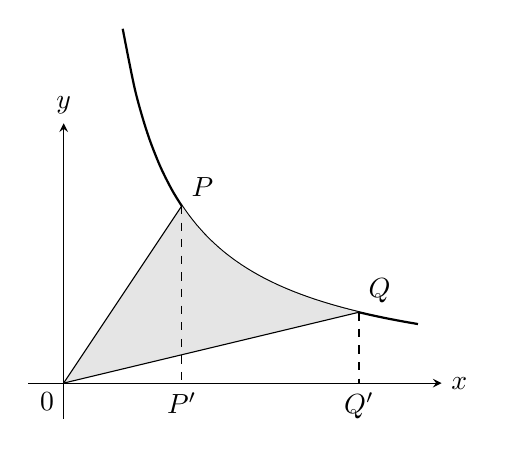
\begin{tikzpicture}[scale=1.5, >=stealth]
  \draw[->] (-0.3, 0) -- (3.2, 0) node[right] {$x$};
  \draw[->] (0, -0.3) -- (0, 2.2) node[above] {$y$};
  \node[below left] at (0,0) {$0$};

  \draw[domain=0.5:3.0, smooth, variable=\x, thick] plot ({\x}, {1.5/\x});

  \coordinate (P) at (1, 1.5);
  \coordinate (Q) at (2.5, 0.6);
  \coordinate (Pp) at (1, 0);
  \coordinate (Qp) at (2.5, 0);

  \fill[gray!20] (0,0) -- (P) -- plot[domain=1:2.5] (\x, {1.5/\x}) -- (Q) -- (0,0);

  \draw (0,0) -- (P) node[above right] {$P$};
  \draw (0,0) -- (Q) node[above right] {$Q$};
  \draw[dashed] (P) -- (Pp) node[below] {$P'$};
  \draw[dashed] (Q) -- (Qp) node[below] {$Q'$};
\end{tikzpicture}
\end{center}

\noindent
\textcircled{1}, \textcircled{2} から
\[
C(t) = \frac{\log t}{\frac{1}{2}\left(t - \frac{1}{t}\right)} = \frac{2t \log t}{t^2 - 1}
\]
\[
C'(t) = \frac{2(\log t + 1)(t^2 - 1) - 2t \log t \cdot 2t}{(t^2 - 1)^2}
\]
\[
= \frac{2}{(t^2 - 1)^2} \left[ -(t^2 + 1)\log t + (t^2 - 1) \right]
\]
\[
= \frac{2(t^2 + 1)}{(t^2 - 1)^2} \left[ -\log t + \frac{t^2 - 1}{t^2 + 1} \right]
\]
この符号は $f(t)$ のそれにひとしい。
ここで $f(t) = -\log t + \frac{t^2 - 1}{t^2 + 1}$ とおくと、
\[
f'(t) = -\frac{1}{t} + \frac{2t(t^2 + 1) - (t^2 - 1)\cdot 2t}{(t^2 + 1)^2}
\]
\[
= \frac{-(t^2 - 1)^2}{t(t^2 + 1)^2} < 0 \quad (\because t > 1)
\]
より、$f(t)$ は単調減少で、$f(t) < f(1) = 0$。よって $C'(t) < 0$ であるから、$C(t)$ は $1 < t$ で単調減少である。 \hfill $\qed$

\bigskip

\subsection*{第4問}

\noindent
\textbf{[解]} $a_1 = 1, a_2 = i \quad \cdots \textcircled{1}, \quad a_{n+2} = a_{n+1} + a_n \quad \cdots \textcircled{2}$

\medskip

\noindent
(1) \textcircled{2} から $a_3 = 1+i, a_4 = 1+2i$ だから、
\[
b_1 = 1-i, \quad b_2 = \frac{1+2i}{1+i} = \frac{3+i}{2}, \quad b_3 = \frac{2+3i}{1+2i} = \frac{8-i}{5}
\]
である。これら3点を通る円の中心は、$b_1 b_2, b_1 b_3$ の垂直2等分線の交点で、
すなわち $\frac{1}{2}$。この時、半径は $\sqrt{\left(1 - \frac{1}{2}\right)^2 + 1^2} = \frac{\sqrt{5}}{2}$ である。

\begin{center}
\begin{tikzpicture}[scale=1.5, >=stealth]
  \draw[->] (-0.5, 0) -- (2.5, 0) node[right] {$\text{Re}$};
  \draw[->] (0, -1.5) -- (0, 1.5) node[above] {$\text{Im}$};
  \node[below left] at (0,0) {$0$};

  \draw[dashed] (0.5, 0) circle (1.118); % radius sqrt(5)/2 approx 1.118

  \fill (1, -1) circle (1.5pt) node[below right] {$b_1$};
  \fill (1.5, 0.5) circle (1.5pt) node[above right] {$b_2$};
  \fill (1.6, -0.2) circle (1.5pt) node[right] {$b_3$};
  \fill (0.5, 0) circle (1.5pt) node[below] {$\frac{1}{2}$};
\end{tikzpicture}
\end{center}

\noindent
(2) 任意の $n \in \mathbb{N}$ に対し、「$b_n$ は円 $C$ の周上にある」$\dots \diamondsuit$ ことを示す。(1)から、$n=1,2,3$ では成立するから、以下 $n=k$ での成立を仮定し ($k \in \mathbb{N}$)、$n=k+1$ での成立を示す。$C$ の中心 $\alpha$, 半径 $r$ とする。
\[
b_{k+1} = \frac{a_{k+2}}{a_{k+1}} = 1 + \frac{a_k}{a_{k+1}} = 1 + \frac{1}{b_k} \quad (\because \textcircled{2})
\]
だから、$b_n \neq 1$ である。逆について
\[
b_k = \frac{1}{b_{k+1}-1} \quad \cdots \textcircled{3}
\]
だから、仮定より $|b_k - \alpha| = r$ に代入、両辺 $0$ 以上から2乗して、
\[
|b_k|^2 - \alpha(b_k + \bar{b}_k) = r^2 - \alpha^2 = 1
\]
両辺 $|b_k|^2 \quad (\neq 0)$ で割って (\textcircled{1}\textcircled{2}から漸化的に $a_n \neq 0$ だから、$b_n \neq 0$ である)、
\[
\frac{1}{|b_k|^2} + \alpha \left( \frac{1}{b_k} + \frac{1}{\bar{b}_k} \right) - 1 = 0
\]
\[
|b_{k+1}-1|^2 + \alpha( \bar{b}_{k+1}-1 + b_{k+1}-1 ) - 1 = 0 \quad (\because \textcircled{3})
\]
\[
|b_{k+1}-1|^2 - \frac{1}{2} ( b_{k+1} + \bar{b}_{k+1} ) - 1 = 0 \quad \left(\because \alpha = \frac{1}{2}\right)
\]
\[
|b_{k+1} - \alpha|^2 = r^2
\]
$|b_{k+1} - \alpha|, r$ 共に $0$ 以上だから、
\[
|b_{k+1} - \alpha| = r
\]
したがって、$b_{k+1}$ も $C$ 上にあるので、$n=k+1$ でも $\diamondsuit$ は成立。よって数学的帰納法により、題意は示された。 \hfill $\text{固}$

\bigskip

\subsection*{第5問}

\noindent
\textbf{[解1]} $x$ [L] の水が入っているビーカーを $X$ とする。又ビーカーに入っている水全質量 $S \quad (S=1)$ とする。

\medskip

\noindent
(1) 命題の否定「$X$ が最後まで残って、かつ水が増えていない」が成立すると仮定する。この時、ビーカーが3個になった時、$X$ は残っており、$x$ (a) (b) の過程で選択されないので、残りのビーカーのには $x$ リットル以下の水しか入っていない。
よって、$S \le 3x < 1$ が成立することになる。これは $S=1$ に矛盾。よって示された。 \hfill $\text{固}$

\medskip

\noindent
(2) 命題の否定「$X$ は (a)(b) の過程で選択される」が成立すると仮定する。
(a)(b) の過程では、3個以上のビーカーの中から、入っている水の量が少ない順に2個のビーカーが選ばれる。よって、$X$ が選ばれる時、$x$ [L] 以上の水が入っているビーカーが $X$ 以外に1個以上存在する。
このようなビーカーが $X$ 以外に2個以上存在すると仮定すると
\[
S \ge 3x > \frac{3}{5}
\]
となり、$S=1$ に矛盾。したがって、$x$ [L] 以上の水が入っているビーカーは $X$ 以外に1個である。それを $Y$ とする。以上の議論より $X$ が選ばれる時、ビーカーは3個であり、その水の量は $y, z, x$ として、$y, z \le x$ と表せる。 $\cdots \star$

ここで、$Y$ は最初からは存在しないから、このビーカーは $x$ リットル以下の水の入った2個のビーカーの水をあわせて作られる。($x$ リットルより多くの水の入ったビーカーが用いられているならば、$x$ リットルのビーカーは残されない)
よって、
\[
y \le 2x
\]
でこの時
\[
S = x + y + z \ge x + \frac{3}{2}y \dots \ge 1
\]
となり、$S=1$ に矛盾。よって示された。 \hfill $\text{固}$

\bigskip

\noindent
\textbf{[解2]}

\medskip

\noindent
(1) 最初に $x$ [L] の水が入っていたビーカーが操作の途中で空になって取り除かれることも、最初より水の量が増えていることもないと仮定する。
水が減る時は、必ず空になり、一度空になったビーカーに水を入れることもないので、この時、最初に $x$ [L] の水が入ったビーカーが存在するので、それぞれ他のビーカーの数量を $x, y, z$ とおける。この時 $x$ [L] の水が入ったビーカーは (a)(b) の対象とならず
\[
y, z \le x
\]
又 $x+y+z = 1$ だから
\[
1 \le 3x \quad \therefore x \ge \frac{1}{3}
\]
これは $x < \frac{1}{3}$ に矛盾。よって示された。 \hfill $\text{固}$

\medskip

\noindent
(2) ($\star$以下) $Y$ [L] のビーカーは最初からは存在しないので、このビーカーがつくられる時を考える。この時、3つのビーカーがあるとし、水量の少ない順に $a_1, a_2, a_3$ とする。又 $x \le \frac{1}{2}$ としても良い。この時、(a)で $a_1, a_2$ が各々選ばれるとして良い。
$a_k$ に入っている水量を $b_k$ とすると、$b_1+b_2 = y \ge x$ だから
\[
b_1+b_2 \ge x \quad \cdots \textcircled{1}
\]
であり、$a_3 \sim a_5$ に入っている水量和は $1-2x$ [L] 以下である。ここから $A$ のビーカーをのぞいたビーカーの内水量の和は $1-2x$ [L] 以下だから、$b_1 \le 1-2x, b_2 \le 1-2x$ となり、
\[
b_1+b_2 \le 2-4x \quad \cdots \textcircled{2}
\]
\textcircled{1}\textcircled{2}から
\[
x \le 2-4x \quad \therefore x \le \frac{2}{5}
\]
これは $x > \frac{2}{5}$ に反し矛盾。したがって示された。 \hfill $\text{固}$

\bigskip

\subsection*{第6問}

\noindent
\textbf{[解]} $A, B$ の $n$ 回目の試行後の座標を $a_n, b_n$ とする。又以下のように場合の数を置く。

\begin{itemize}
  \item[$1^\circ$] $a_n > b_n \quad (P_n)$ \\
  表なら共に $+1$、裏なら $B$ を $+1$ すすめる。
  \item[$2^\circ$] $a_n = b_n \quad (X_n)$ \\
  表なら $A$ を $+1$ すすめる、裏なら $B$ を $+1$ すすめる。
  \item[$3^\circ$] $a_n < b_n \quad (Q_n)$ \\
  表なら $A$ を $+1$ すすめる、裏なら共に $+1$ すすめる。
\end{itemize}

\medskip

\noindent
(1) 題意から、任意の $n$ に対して、$|a_n - b_n| \le 1$ である。したがって $n+1$ 回目に $a_{n+1} = b_{n+1}$ となるのは以下の場合：
\[
\begin{cases}
1^\circ \text{ で裏が出る。} \\
3^\circ \text{ で表が出る。}
\end{cases}
\]
したがって、
\[
X_{n+1} = P_n + Q_n = 2^n - X_n \quad (\because P_n + Q_n + X_n = 2^n) \quad \cdots \textcircled{1}
\]

\medskip

\noindent
(2) $Y_n = \frac{X_n}{2^n}$ によって $\{Y_n\}$ を定める。\textcircled{1}の両辺を $2^{n+1}$ でわって
\[
Y_{n+1} = -\frac{1}{2}Y_n + \frac{1}{2}
\]
\[
Y_{n+1} - \frac{1}{3} = -\frac{1}{2}\left(Y_n - \frac{1}{3}\right) \quad \cdots \textcircled{2}
\]
$X_1 = 0$ つまり $Y_1 = 0$ だから、\textcircled{2}をくり返し用いて、
\[
Y_n - \frac{1}{3} = \left(-\frac{1}{2}\right)^{n-1}\left(-\frac{1}{3}\right)
\]
\[
\therefore X_n = \frac{1}{3} \{ 2^n + 2 \cdot (-1)^n \} \hfill \text{\slash\slash}
\]

\medskip

\noindent
(3) $A_n$ の期待値 $E_n(a)$ を求めれば良い。ここで、確率変数 $t_k$ を以下のように定める。
\[
t_k = \begin{cases}
0 & (k \text{回目の試行で } A \text{ が進まない}) \\
1 & (k \text{回目の試行で } A \text{ が進む})
\end{cases}
\]
すると、題意から
\[
E_n(a) = \sum_{k=1}^n P(t_k = 1) \quad \cdots \textcircled{3}
\]
である。$k$ 回目で $A$ が進むのは以下の時：
\[
\begin{cases}
\text{\textcircled{1} コインで表が出る。 (確率 } \frac{1}{2}\text{)} \\
\text{\textcircled{2} } a_{k-1} < b_{k-1} \text{ かつ コインで裏が出る。}
\end{cases}
\]
ここで、(1)及び(2)、対称性から $P_n = Q_n$ であることから、
\[
P_n = \frac{1}{2} (2^n - X_n) = \frac{1}{3} (2^n - (-1)^n)
\]
だから、\textcircled{2}の起きる確率は $\frac{1}{2^k} P_{k-1}$ である。したがって、$k \ge 2$ の時、
\[
P(t_k = 1) = \frac{1}{2} + \frac{1}{2^k} \cdot \frac{1}{3} ( 2^{k-1} - (-1)^{k-1} ) = \frac{2}{3} + \frac{1}{3} \left(-\frac{1}{2}\right)^k
\]
である。$k=1$ の時、$P(t_1=1) = \frac{1}{2}$ であるからこれも良い。したがって\textcircled{3}から、
\[
E_n(a) = \sum_{k=1}^n \left\{ \frac{2}{3} + \frac{1}{3}\left(-\frac{1}{2}\right)^k \right\}
\]
\[
= \frac{2}{3}n - \frac{1}{6} \cdot \frac{1 - (-1/2)^n}{1 + 1/2} = \frac{2}{3}n - \frac{1}{9}\left\{ 1 - \left(-\frac{1}{2}\right)^n \right\} \hfill \text{\slash\slash}
\]

\end{document}
